% 	Name		:: 	BDEEP template is based on the sthlm theme (Mark Hendry Olson (mark@hendryolson.com))
%	Author		:: 	Peter Christensen
%	Created		::	2016-04-12
%	Updated		::	June 18, 2015 at 08:45
%	Version		:: 	1.0
%	Email		:: 	pchrist@illinois.edu
%	Website		:: 	bdeep webiste
%
% 	License		:: 	This file may be distributed and/or modified under the
%                  	GNU Public License.
%
%	Description	::	This template makes use of the Stockholm theme from Mark Hendry Olson and includes items and files necessary for creating presentations on behalf of our group.


%-=-=-=-=-=-=-=-=-=-=-=-=-=-=-=-=-=-=-=-=-=-=-=-=
%
%        LOADING DOCUMENT
%
%-=-=-=-=-=-=-=-=-=-=-=-=-=-=-=-=-=-=-=-=-=-=-=-=

\documentclass[newPxFont]{beamer}
\usetheme{sthlm}
%\usecolortheme{sthlmv42}

%-=-=-=-=-=-=-=-=-=-=-=-=-=-=-=-=-=-=-=-=-=-=-=-=
%        LOADING PACKAGES
%-=-=-=-=-=-=-=-=-=-=-=-=-=-=-=-=-=-=-=-=-=-=-=-=
\usepackage[utf8]{inputenc}

\usepackage{chronology}

\renewcommand{\event}[3][e]{%
  \pgfmathsetlength\xstop{(#2-\theyearstart)*\unit}%
  \ifx #1e%
    \draw[fill=black,draw=none,opacity=0.5]%
      (\xstop, 0) circle (.2\unit)%
      node[opacity=1,rotate=45,right=.2\unit] {#3};%
  \else%
    \pgfmathsetlength\xstart{(#1-\theyearstart)*\unit}%
    \draw[fill=black,draw=none,opacity=0.5,rounded corners=.1\unit]%
      (\xstart,-.1\unit) rectangle%
      node[opacity=1,rotate=45,right=.2\unit] {#3} (\xstop,.1\unit);%
  \fi}%

%-=-=-=-=-=-=-=-=-=-=-=-=-=-=-=-=-=-=-=-=-=-=-=-=
%        BEAMER OPTIONS
%-=-=-=-=-=-=-=-=-=-=-=-=-=-=-=-=-=-=-=-=-=-=-=-=

\setbeameroption{show notes}

%-=-=-=-=-=-=-=-=-=-=-=-=-=-=-=-=-=-=-=-=-=-=-=-=
%
%	PRESENTATION INFORMATION
%
%-=-=-=-=-=-=-=-=-=-=-=-=-=-=-=-=-=-=-=-=-=-=-=-=

\title{Big Data and Big Challenges:}
\subtitle{Addressing Urban Transportation and Congestion in Developing Countries}
\date{4/13/2016}
\author{Peter Christensen}
\institute{University of Illinois}


\begin{document}

%-=-=-=-=-=-=-=-=-=-=-=-=-=-=-=-=-=-=-=-=-=-=-=-=
%
%	TITLE PAGE
%
%-=-=-=-=-=-=-=-=-=-=-=-=-=-=-=-=-=-=-=-=-=-=-=-=

\maketitle

%\begin{frame}[plain]
%	\titlepage
%\end{frame}

%-=-=-=-=-=-=-=-=-=-=-=-=-=-=-=-=-=-=-=-=-=-=-=-=
%
%	TABLE OF CONTENTS: OVERVIEW
%
%-=-=-=-=-=-=-=-=-=-=-=-=-=-=-=-=-=-=-=-=-=-=-=-=

\section*{Introduction}

%-=-=-=-=-=-=-=-=-=-=-=-=-=-=-=-=-=-=-=-=-=-=-=-=
%	FRAME: Introduction
%-=-=-=-=-=-=-=-=-=-=-=-=-=-=-=-=-=-=-=-=-=-=-=-=


\begin{frame}[c]{How Big is the Congestion Problem?}
	We know that this is an economically important problem in the United States
	\begin{columns}
		\begin{column}{.5\linewidth}
			\begin{enumerate}   
				\item{Primary Impacts on the Economy}
				\begin{itemize}  
					\item{Cost of Time}
					\item{Cost of Emissions}
					\item{Cost of Accidents}
				\end{itemize}  
			\end{enumerate}
		\end{column}
		\begin{column}{.49\linewidth}
			\begin{figure}
				\centering
				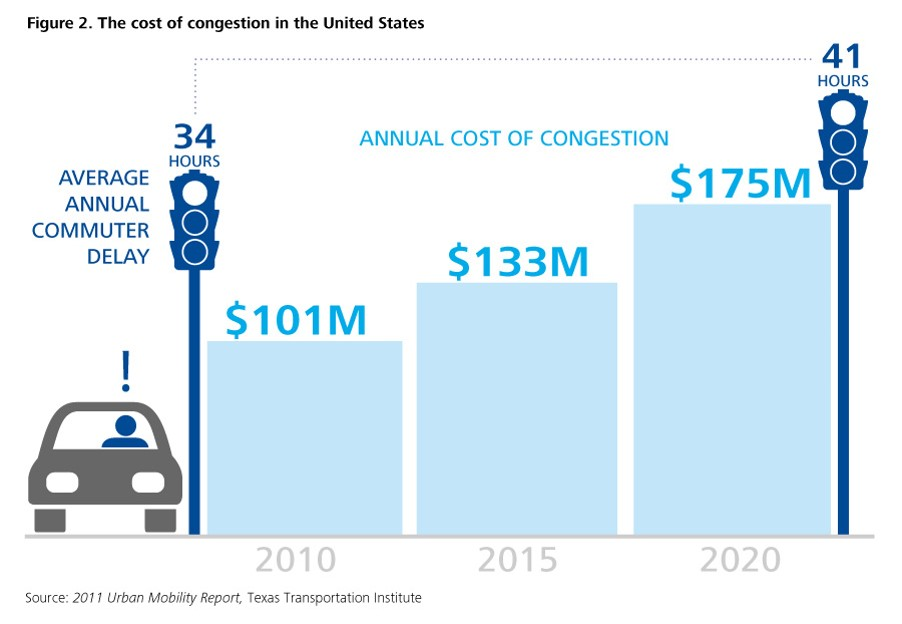
\includegraphics[width=1.1\linewidth]{USCongestion.jpg}
			\end{figure}
		\end{column}
	\end{columns}
\end{frame}

%-=-=-=-=-=-=-=-=-=-=-=-=-=-=-=-=-=-=-=-=-=-=-=-=
%	FRAME: Introduction
%-=-=-=-=-=-=-=-=-=-=-=-=-=-=-=-=-=-=-=-=-=-=-=-=


\begin{frame}[c]{The Congestion Problem in Developing Countries}
	The costs are much higher. How High?
	\begin{enumerate}   
		\item{Rough estimates for a few cities}
		\begin{itemize}  
			\item{Beijing -- 2009 study estimated the economic cost of congestion for a Beijing resident ay 335.6 CNY per month (\$50 US)}
			\item{Bijing's population is ~20 Million, so the total cost approaches \$12 Billion}
			\item{Cairo -- one study estimates \$8 Billion}
		\end{itemize}  
	\end{enumerate}
	\begin{figure}
		\centering
		\includegraphics[width=.6\linewidth]{traffic.png}
	\end{figure}
\end{frame}

%-=-=-=-=-=-=-=-=-=-=-=-=-=-=-=-=-=-=-=-=-=-=-=-=
%	FRAME: Introduction
%-=-=-=-=-=-=-=-=-=-=-=-=-=-=-=-=-=-=-=-=-=-=-=-=


\begin{frame}[c]{Why is it Important to Estimate these Costs?}
	This is not simply an economic exercise.  These figures drive real policy decisions amidst competing priorities
	\begin{enumerate}   
		\item{Investments in new transportation infrastructure}
		\item{Investments in public transportation services}
		\item{Air pollution abatement}
		\item{International lending and aid projects}
		\item{Traffic regulations, restrictions and subsidies}
	\end{enumerate}
	\begin{figure}
		\centering
		\includegraphics[width=.6\linewidth]{traffic.png}
	\end{figure}
\end{frame}



\section*{Overview}
\begin{frame}{Overview}
% For longer presentations use hideallsubsections option
\tableofcontents[hideallsubsections]
\end{frame}


%-=-=-=-=-=-=-=-=-=-=-=-=-=-=-=-=-=-=-=-=-=-=-=-=
%
%	SECTION: BACKGROUND
%
%-=-=-=-=-=-=-=-=-=-=-=-=-=-=-=-=-=-=-=-=-=-=-=-=

\section{Economics of Congestion: Background}

%-=-=-=-=-=-=-=-=-=-=-=-=-=-=-=-=-=-=-=-=-=-=-=-=
%	FRAME: Slide with Graphic/Text
%-=-=-=-=-=-=-=-=-=-=-=-=-=-=-=-=-=-=-=-=-=-=-=-=
\begin{frame}[c]{Classic Externalities}
Social costs of traffic congestion are a classic externality
\begin{enumerate}  
	\item{An individual's use of transport infrastructure impose social costs on other individuals}
	\item{We consume up to Q1 when it is optimal to consume to Q2}  
	\item{Regulations are used to correct the market failure}
\end{enumerate}
\begin{figure}
	\centering
	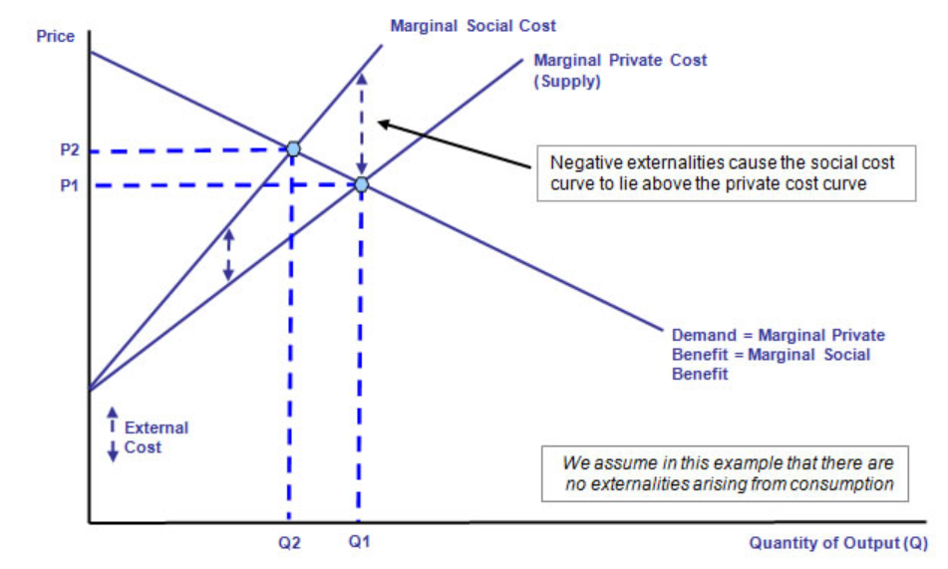
\includegraphics[width=0.65\linewidth]{P_QGraph.png}
\end{figure}  
\end{frame}

%-=-=-=-=-=-=-=-=-=-=-=-=-=-=-=-=-=-=-=-=-=-=-=-=
%	FRAME: Slide with Graphic/Text
%-=-=-=-=-=-=-=-=-=-=-=-=-=-=-=-=-=-=-=-=-=-=-=-=
\begin{frame}[c]{Types of Regulation}
	Transport regulations change behavior through effects on:
	\begin{columns}
		\begin{column}{.5\linewidth}
	\begin{enumerate}  
		\item{Prices (P1 -> P2)}
		\begin{itemize} 
			\item{congestion pricing} 
			\item{subsidies to mass transit}
			\item{gasoline tax} 
		\end{itemize}
		\item{Quantities (Q1 -> Q2)}
		\begin{itemize} 
			\item{driving restrictions} 
			\item{license plate lotteries}
		\end{itemize}
	\end{enumerate}
		\end{column}
		
		\begin{column}{.5\linewidth}
	\begin{figure}
		\centering
		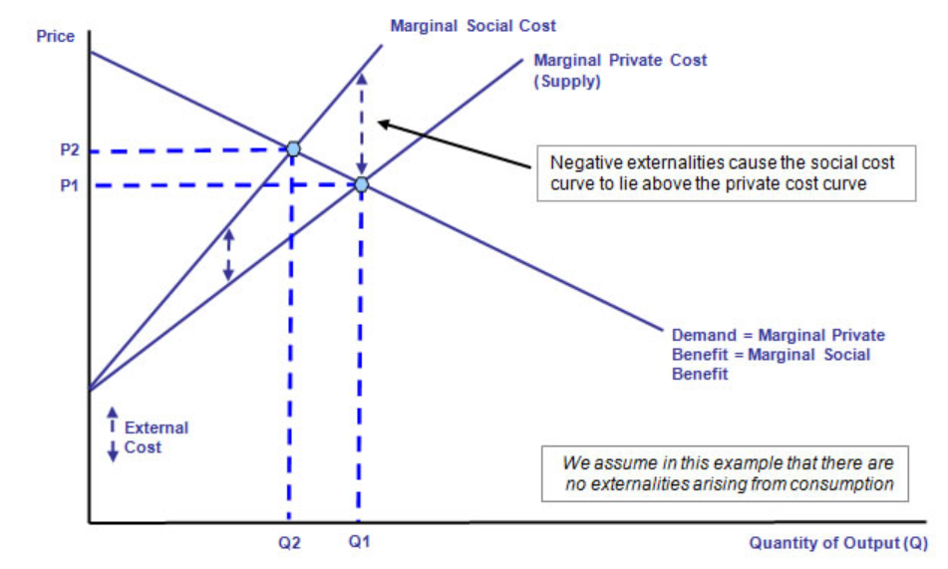
\includegraphics[width=1.0\linewidth]{P_QGraph.png}
	\end{figure}  
		\end{column}
	\end{columns}
\end{frame}

%-=-=-=-=-=-=-=-=-=-=-=-=-=-=-=-=-=-=-=-=-=-=-=-=
%	FRAME: Slide with Graphic Column and Text Column
%-=-=-=-=-=-=-=-=-=-=-=-=-=-=-=-=-=-=-=-=-=-=-=-=
\begin{frame}[c]{Blind Experiments with Regulations}
	\begin{columns}
		\begin{column}{.53\linewidth}
			\begin{enumerate}   
				\item{Driving Restrictions}
				\begin{itemize}
					\item{Most recent experiment: New Delhi}  
					\item{Existing in: Mexico City, Sao Paulo, Beijing, Shanghai}
				\end{itemize}  
			\end{enumerate}
		\end{column}
		\begin{column}{.45\linewidth}
			\begin{figure}
				\centering
				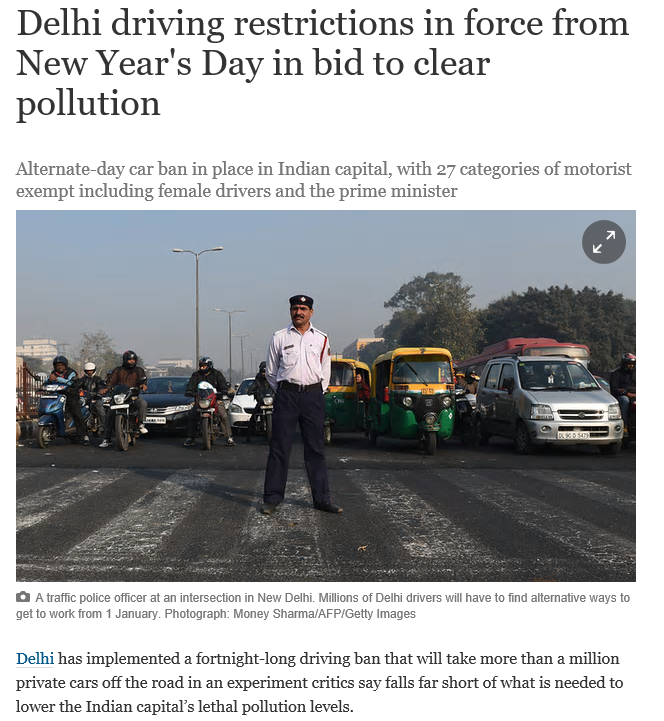
\includegraphics[width=1.05\linewidth]{Delhi.png}
			\end{figure}
		\end{column}
	\end{columns}
\end{frame}

%-=-=-=-=-=-=-=-=-=-=-=-=-=-=-=-=-=-=-=-=-=-=-=-=
%	FRAME: Slide with Graphic Column and Text Column
%-=-=-=-=-=-=-=-=-=-=-=-=-=-=-=-=-=-=-=-=-=-=-=-=
\begin{frame}[c]{Limited Evidence from Mexico City}
	\begin{columns}
		\begin{column}{.53\linewidth}
			\begin{figure}
				\centering
				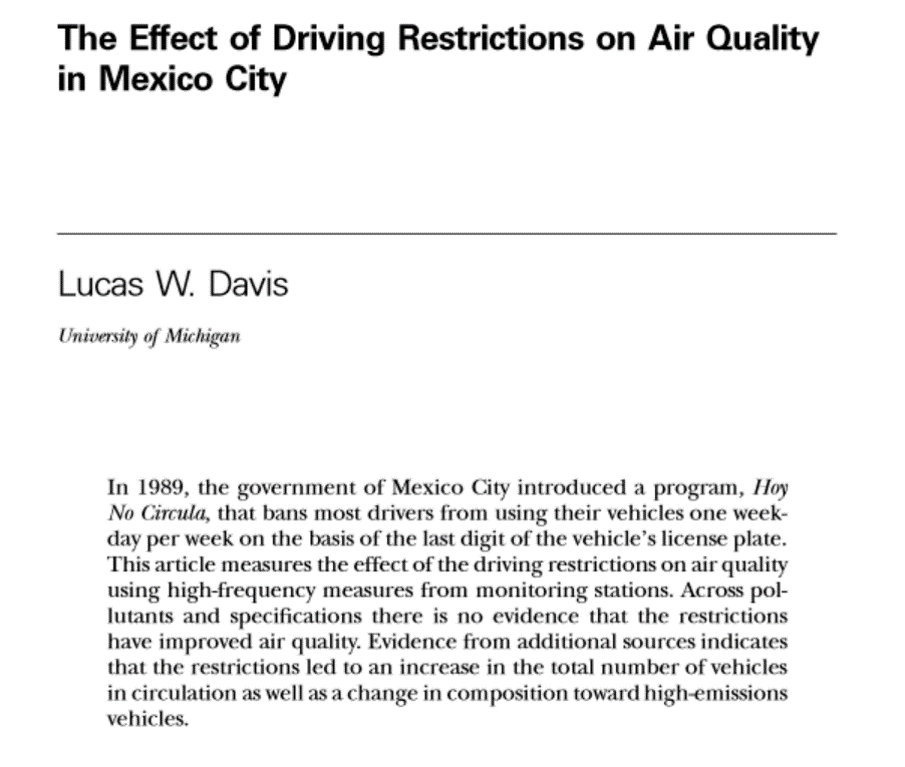
\includegraphics[width=1.2\linewidth]{Davis_paper.png}
			\end{figure} 

		\end{column}
		\begin{column}{.45\linewidth}
			\begin{figure}
				\centering
				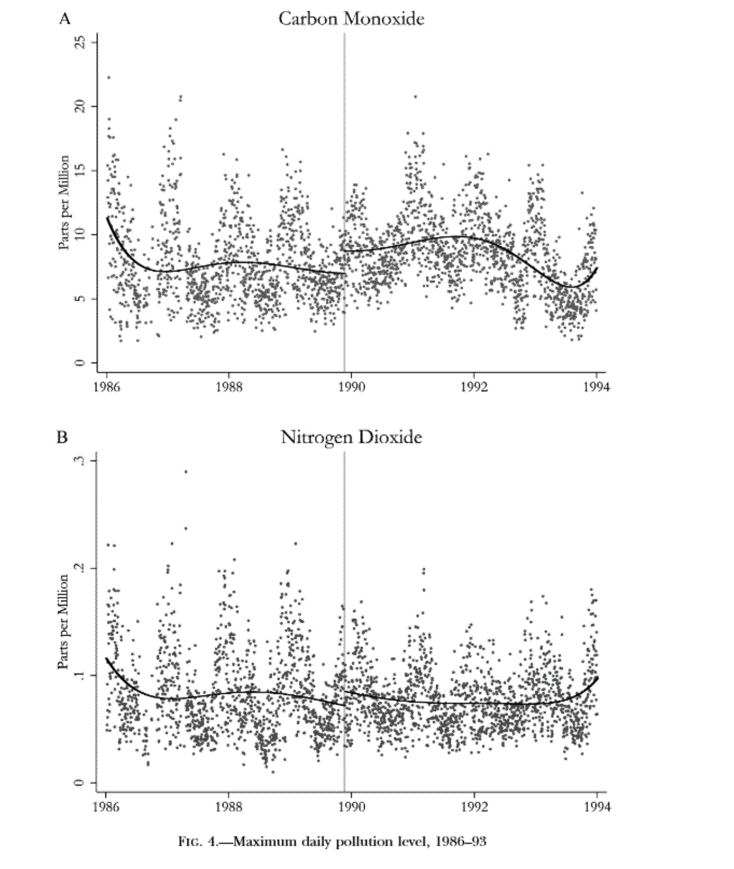
\includegraphics[width=1.05\linewidth]{Davis_graph.png}
			\end{figure}
		\end{column}
	\end{columns}
\end{frame}

%-=-=-=-=-=-=-=-=-=-=-=-=-=-=-=-=-=-=-=-=-=-=-=-=
%	FRAME: Slide with Items and Subitems
%-=-=-=-=-=-=-=-=-=-=-=-=-=-=-=-=-=-=-=-=-=-=-=-=
\begin{frame}[c]{Research Questions}
	Primary Questions	
	\begin{enumerate}   
		\item{What is the cost of traffic congestion in developing country cities}  
		\begin{itemize}
			\item{Total cost to society}
			\item{Marginal cost -- how much does society benefit from 1 minute less spend in traffic?}
		\end{itemize}
		\item{What are the impacts of regulatory changes on social welfare?}
		\begin{itemize}
			\item{How do costs respond to driving restrictions?}
			\item{How do costs respond to mass transit subsidies?}
		\end{itemize}
	\end{enumerate}	
\end{frame}

%-=-=-=-=-=-=-=-=-=-=-=-=-=-=-=-=-=-=-=-=-=-=-=-=
%
%	SECTION: DATA AND METHODOLOGY
%
%-=-=-=-=-=-=-=-=-=-=-=-=-=-=-=-=-=-=-=-=-=-=-=-=

\section{Data and Method}
%-=-=-=-=-=-=-=-=-=-=-=-=-=-=-=-=-=-=-=-=-=-=-=-=
%	FRAME: Transit Demand
%-=-=-=-=-=-=-=-=-=-=-=-=-=-=-=-=-=-=-=-=-=-=-=-=
\begin{frame}[c]{Transit Demand}
Demand for transit is estimated using a model of consumer utility:\\
	\begin{equation}{\label{eq1}}
	U=X-\alpha(T(V),C,D)  
	\end{equation}
	X = consumption of an outside composite good\\
	$\alpha$ = cost of a trip, which depends on the distance (D) of the trip, its monetary cost (C), its duration (T), and the individual's value of time (V)\\
	
	\begin{itemize}
		\item{we assume that consumers are optimizing}
		\item{consumers can substitute across modes, times, or forgo trips altogether}
	\end{itemize}

\end{frame}


%-=-=-=-=-=-=-=-=-=-=-=-=-=-=-=-=-=-=-=-=-=-=-=-=
%	FRAME: Slide with Itemized Text and Graphics Columns
%-=-=-=-=-=-=-=-=-=-=-=-=-=-=-=-=-=-=-=-=-=-=-=-=
\begin{frame}[c]{Data Sources}
	\begin{columns}
		\begin{column}{.5\linewidth}
			\begin{figure}
				\centering
				
\includegraphics[width=0.6\linewidth]{survey.jpg}
			\end{figure}
		\end{column}
		\begin{column}{.5\linewidth}
			\begin{figure}
				\centering
				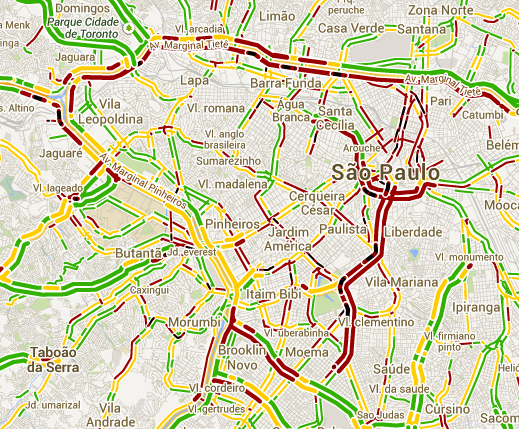
\includegraphics[width=0.7\linewidth]{SaoPaoloGoogle.png}
			\end{figure}
		\end{column}
	\end{columns}
	\begin{enumerate}
		\item{City Level Trip Surveys: representative sample of travel for a week of travel in a city}\\
		\begin{itemize}
			\item{origin/destination, day/time, mode, monetary cost of trip}
			\item{residence, car ownership, income, purpose of trip}
		\end{itemize}
		\item{Google Traffic API: simulate entire set of trips each week}\\
		\begin{itemize}
			\item{duration of trip in traffic, duration with no congestion (2am), duration using alternative times/modes}
		\end{itemize}
	\end{enumerate}
\end{frame}

%-=-=-=-=-=-=-=-=-=-=-=-=-=-=-=-=-=-=-=-=-=-=-=-=
%	FRAME: Slide with Equations and Text
%-=-=-=-=-=-=-=-=-=-=-=-=-=-=-=-=-=-=-=-=-=-=-=-=
\begin{frame}{Weekly Estimates of Impact of Congestion on Welfare}
	Structural estimates of the value of time for and individual taking each trip
	\begin{equation}{\label{eq1}}
	CS = \sum\limits_{N=1}^{50,000}V_{i,t}   
	\end{equation}
	Text pertaining to euqation 1 with imbedded notation: ($C^{\tau}$).
	\begin{equation}{\label{eq2}}
	L_{it}^{u}=f(V_{it}^{a},C_{it}^{a},C^{\tau})
	\end{equation}
\end{frame}

%-=-=-=-=-=-=-=-=-=-=-=-=-=-=-=-=-=-=-=-=-=-=-=-=
%	FRAME: Slide with Text, Equation, and Figure/Graphic
%-=-=-=-=-=-=-=-=-=-=-=-=-=-=-=-=-=-=-=-=-=-=-=-=

\begin{frame}{Slide with Text, Equation, and Figure/Graphic}
	Equation 1:
	\begin{equation}{\label{eq2}}
		\tau_{ATT(\frac{da}{du})}=[\frac{dL^{a}}{dL^{u}}_{it}(1)-\frac{dL^{a}}{dL^{u}}_{it}(0)]
	\end{equation}
	\begin{figure}
		\centering
		\includegraphics[width=0.6\linewidth, trim=0 0 0 400, clip]{CompareHiRes_Guangzhou.eps}
	\end{figure}
\end{frame}

%-=-=-=-=-=-=-=-=-=-=-=-=-=-=-=-=-=-=-=-=-=-=-=-=
%	FRAME: Slide with Annotated Timeline
%-=-=-=-=-=-=-=-=-=-=-=-=-=-=-=-=-=-=-=-=-=-=-=-=


\begin{frame}[c]{Slide with Annotated Timeline}
	\vspace{-1cm}
	\begin{center}\begin{chronology}[5]{1988}{2005}{0.85\textwidth}
			\event[\decimaldate{1}{1}{1990}]{\decimaldate{1}{11}{1994}}{\cRed{Period 1 in red}}
			\event[\decimaldate{1}{3}{1995}]{\decimaldate{1}{11}{1999}}{ 1997 - No Net Loss Regulation}
			\event[\decimaldate{1}{3}{2000}]{\decimaldate{1}{1}{2005}}{\cRed{Period 2 in red}}
		\end{chronology}
	\end{center}
	
\end{frame}


%-=-=-=-=-=-=-=-=-=-=-=-=-=-=-=-=-=-=-=-=-=-=-=-=
%
%	SECTION: RESULTS
%
%-=-=-=-=-=-=-=-=-=-=-=-=-=-=-=-=-=-=-=-=-=-=-=-=
\section{Results}

%-=-=-=-=-=-=-=-=-=-=-=-=-=-=-=-=-=-=-=-=-=-=-=-=
%	FRAME: Results-Type Slide
%-=-=-=-=-=-=-=-=-=-=-=-=-=-=-=-=-=-=-=-=-=-=-=-=

\begin{frame}[c]{Results-Type Slide}
	Primary Findings	
	\begin{enumerate}   
		\item{First Item}
		\begin{itemize}
			\item{first subitem}
			\item{second subitem (remember that percentages must be coded correctly 50\%).}
			\item{third subitem}
			\item{fourth subitem}
		\end{itemize}
	\end{enumerate}	
\end{frame}

%-=-=-=-=-=-=-=-=-=-=-=-=-=-=-=-=-=-=-=-=-=-=-=-=
%
%	SECTION: CONCLUSIONS
%
%-=-=-=-=-=-=-=-=-=-=-=-=-=-=-=-=-=-=-=-=-=-=-=-=
\section{Conclusions}

%-=-=-=-=-=-=-=-=-=-=-=-=-=-=-=-=-=-=-=-=-=-=-=-=
%	FRAME: Conclusions
%-=-=-=-=-=-=-=-=-=-=-=-=-=-=-=-=-=-=-=-=-=-=-=-=

\begin{frame}[c]{Conclusions}
	Heading
	\begin{enumerate}   
		\item{Item 1}  
		\begin{itemize}
			\item{subitem 1}
			\item{subitem 2}
			\item{subitem 3}
		\end{itemize}
		\item{Item 2}
		\begin{itemize}
			\item{subitem 1}
			\item{subitem 2}
			\item{subitem 3}
		\end{itemize}
	\end{enumerate}	
\end{frame}

%-=-=-=-=-=-=-=-=-=-=-=-=-=-=-=-=-=-=-=-=-=-=-=-=
%
%	SECTION: LINKS AND ACKNOWLEDGEMENTS
%
%-=-=-=-=-=-=-=-=-=-=-=-=-=-=-=-=-=-=-=-=-=-=-=-=

\begin{frame}{Links and Acknowledgements}
	
You can find publications at \url{www.peterchristensen.net}.\\
\vspace{1em}
If you are interested in learning about the technology that we are building to support our economics and policy research, please come find us on the 3rd floor of the National Center for Supercomputing Applications (NCSA).\\
\vspace{1em}	
Please send questions and comments to: pchrist@illinois.edu
\end{frame}

\end{document}
